\title[ASD - Analisi di algoritmi]{\textbf{Algoritmi e Strutture Dati}\\[18pt]Analisi di algoritmi\\Proprietà della notazione asintotica}

%-------------------------------------------------------------------------
\FrameTitle{}

%%%%%%%%%%%%%%%%%%%%%%%%%%%%%%%%%%%%%%%%%%%%%%%%%%%%%%%%%%%%%%%%%%%%%%%%%%
\section{Proprietà della notazione asintotica}

\subsection{Funzioni di costo particolari}
\begin{frame}{Regola generale}

\begin{myboxtitle}[Espressioni polinomiali]
$
  \alert{f(n) = a_k n^k + a_{k-1}n^{k-1} + \ldots a_1 n + a_0, a_k >0 \Rightarrow f(n) = \Theta(n^k)}  
$
\end{myboxtitle}

\begin{overprint}
\onslide<1|handout:1>
\textbf{Limite superiore}: $\exists c>0, \exists m \geq 0: f(n) \leq cn^k, \forall n \geq m$

\begin{align*}
f(n) &= a_kn^k + a_{k-1}n^{k-1} +  \ldots  + a_1n + a_0 \\
     &\leq a_kn^k + |a_{k-1}|n^{k-1} +  \ldots  + |a_1|n + |a_0| \\
     &\leq a_kn^k + |a_{k-1}|n^k +  \ldots  + |a_1|n^k + |a_0|n^k && \forall n \geq 1\\
     &= (a_k + |a_{k-1}| +  \ldots  + |a_1| + |a_0|)n^k \\
     &\stackrel{?}{\leq} cn^k
\end{align*}
che è vera per $c \geq (a_k + |a_{k-1}| +  \ldots  + |a_1| + |a_0|) > 0$ e per $m = 1$.
\onslide<2|handout:2>
\textbf{Limite inferiore}: $\exists d>0, \exists m \geq 0: f(n) \geq dn^k, \forall n \geq m$

\begin{align*}
f(n) &= a_kn^k + a_{k-1}n^{k-1} +  \ldots  + a_1n + a_0 \\
     &\geq a_kn^k - |a_{k-1}|n^{k-1} - \ldots  - |a_1|n - |a_0| \\
     &\geq a_kn^k - |a_{k-1}|n^{k-1} - \ldots  - |a_1|n^{k-1} - |a_0|n^{k-1} && \forall n \geq 1\\
     &\stackrel{?}{\geq} dn^k
\end{align*}
L'ultima equazione è vera se:
\[
  d \leq a_k - \frac{|a_{k-1}|}{n} - \frac{|a_{k-2}|}{n} -\ldots  - \frac{|a_1|}{n} - \frac{|a_0|}{n} > 0 \Leftrightarrow 
  n > \frac{|a_{k-1}| + \ldots + | a_0 |}{a_k}
\]
\end{overprint}
\end{frame}

\begin{frame}{Alcuni casi particolari}
\begin{itemize}
\item Qual è la complessità di \alert{$f(n) = 5$}?
  \pause
  \begin{itemize}
	 \item $f(n) = 5 \geq c_1 n^0 \Rightarrow c_1 \leq 5$
	 \item $f(n) = 5 \leq c_2 n^0 \Rightarrow c_2 \geq 5$
	 \item $f(n) = \Theta(n^0) = \Theta(1)$
  \end{itemize}
\pause
\item Qual è la complessità di \alert{$f(n) = 5+\sin(n)$}?
  \pause
  \alert{$\Theta(1)$}
  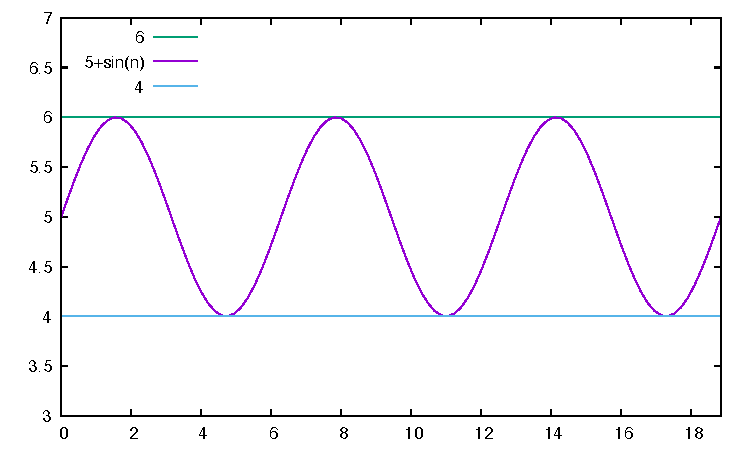
\includegraphics[width=0.5\textwidth]{plot-2}  
\end{itemize}
\end{frame}

\subsection{Proprietà delle notazioni}

\begin{frame}{Proprietà}

\begin{myboxtitle}[Dualità]
\[
	f(n) = O(g(n)) \Leftrightarrow g(n) = \Omega(f(n)) 
\]
\end{myboxtitle}

Dimostrazione:

\begin{align*}
f(n) = O(g(n)) 	& \Leftrightarrow f(n) \leq cg(n), \forall n\geq m \\
				& \Leftrightarrow g(n) \geq \frac{1}{c} f(n), \forall n \geq m \\
				& \Leftrightarrow g(n) \geq c' f(n), \forall n \geq m, c' = \frac{1}{c} \\
				& \Leftrightarrow g(n) = \Omega(f(n))
\end{align*}

\end{frame}

\begin{frame}{Proprietà}

\begin{myboxtitle}[Eliminazione delle costanti]
\begin{align*}
  f(n) = O(g(n)) &\Leftrightarrow af(n) = O(g(n)), \forall a>0 \\
  f(n) = \Omega(g(n)) &\Leftrightarrow af(n) = \Omega(g(n)), \forall a>0 
\end{align*}
\end{myboxtitle}

Dimostrazione:

\begin{align*}
  f(n) = O(g(n)) &\Leftrightarrow f(n) \leq cg(n), \forall n \geq m \\
                 &\Leftrightarrow af(n) \leq acg(n), \forall n \geq m, \forall a \geq 0 \\
                 &\Leftrightarrow af(n) \leq c'g(n), \forall n \geq m, c' = ac > 0 \\
                 &\Leftrightarrow af(n) = O(g(n))
\end{align*}

\end{frame}

\begin{frame}{Proprietà}

\begin{myboxtitle}[Sommatoria (sequenza di algoritmi)]
\small
\begin{align*}
  f_1(n) = O(g_1(n)), f_2(n) = O(g_2(n)) &\Rightarrow f_1(n)+f_2(n) = O(\max(g_1(n), g_2(n))) \\
  f_1(n) = \Omega(g_1(n)), f_2(n) = \Omega(g_2(n)) &\Rightarrow f_1(n)+f_2(n) = \Omega(\max(g_1(n), g_2(n))) 
\end{align*}
\end{myboxtitle}

\begin{myboxtitle}[Dimostrazione (Lato $O$)]
\begin{eqnarray*}
  f_1(n) = O(g_1(n)) \wedge f_2(n) = O(g_2(n)) &\Rightarrow& \\
    f_1(n) \leq c_1g_1(n) \wedge f_2(n) \leq c_2g_2(n) &\Rightarrow& \\
    f_1(n)+f_2(n) \leq c_1g_1(n) + c_2g_2(n) &\Rightarrow& \\
    f_1(n)+f_2(n) \leq \max\{c_1,c_2\} (2 \cdot \max(g_1(n),g_2(n))) &\Rightarrow& \\
    f_1(n)+f_2(n) = O(\max(g_1(n), g_2(n)))
\end{eqnarray*}
\end{myboxtitle}

\end{frame}

\begin{frame}{Proprietà}

\begin{myboxtitle}[Prodotto (Cicli annidati)]
\small
\begin{align*}
  f_1(n) = O(g_1(n)), f_2(n) = O(g_2(n)) &\Rightarrow f_1(n) \cdot f_2(n) = O(g_1(n) \cdot g_2(n)) \\
  f_1(n) = \Omega(g_1(n)), f_2(n) = \Omega(g_2(n)) &\Rightarrow f_1(n) \cdot f_2(n) = \Omega(g_1(n) \cdot g_2(n)) 
\end{align*}
\end{myboxtitle}

\begin{myboxtitle}[Dimostrazione]
\begin{eqnarray*}
  f_1(n) = O(g_1(n)) \wedge f_2(n) = O(g_2(n)) &\Rightarrow& \\
    f_1(n) \leq c_1g_1(n) \wedge f_2(n) \leq c_2g_2(n) &\Rightarrow& \\
    f_1(n) \cdot f_2(n) \leq c_1c_2g_1(n)g_2(n)  
\end{eqnarray*}
\end{myboxtitle}

\end{frame}

\begin{frame}{Proprietà}

\begin{myboxtitle}[Simmetria]
	\[
	f(n) = \Theta(g(n)) \Leftrightarrow g(n) = \Theta(f(n))
	\]
\end{myboxtitle}

\begin{myboxtitle}[Dimostrazione]
Grazie alla proprietà di dualità:

\begin{eqnarray*}
  f(n) = \Theta(g(n)) &\Rightarrow& f(n) = O(g(n)) \Rightarrow g(n) = \Omega(f(n)) \\
  f(n) = \Theta(g(n)) &\Rightarrow& f(n) = \Omega(g(n)) \Rightarrow g(n) = O(f(n)) \\
\end{eqnarray*}
\end{myboxtitle}

\end{frame}

\begin{frame}{Proprietà}

\begin{myboxtitle}[Transitività]
\[
  f(n) = O(g(n)), g(n) = O(h(n)) \Rightarrow f(n) = O(h(n))
\]
\end{myboxtitle}

\begin{myboxtitle}[Dimostrazione]
\begin{eqnarray*}
  f(n) = O(g(n)) \wedge g(n) = O(h(n)) &\Rightarrow& \\
    f(n) \leq c_1g(n) \wedge g(n) \leq c_2h(n) &\Rightarrow& \\
    f(n) \leq c_1c_2h(n)  &\Rightarrow& \\
    f(n) = O(h(n)) &&
\end{eqnarray*}
\end{myboxtitle}

\end{frame}

\subsection{Altre funzioni di costo}

\begin{frame}[shrink]{Logaritmi vs funzioni lineari}

\begin{myboxtitle}[Proprietà dei logaritmi]
Vogliamo provare che \alert{$\log n = O(n)$}. Dimostriamo per induzione che\\[-6pt]
\[
\exists c>0, \exists m \geq 0: \alert{\log n \leq cn}, \forall n \geq m
\]	
	% \[
	%    \log n = O(n)
	% \]
\end{myboxtitle}
%
% Dimostriamo per induzione che $\exists c>0, \exists m \geq 0: \alert{\log n \leq cn}, \forall n \geq m$
\begin{overprint}
\onslide<1|handout:1>
  \begin{itemize}
  \item \textbf{Caso base ($n=1$)}: 
     \[
       \log 1 = 0 \leq cn = c \cdot 1 \Leftrightarrow c \geq 0
     \]
  \end{itemize}
\onslide<2|handout:2>
  \begin{itemize}
  \item \textbf{Ipotesi induttiva}: sia \alert{$\log k \leq ck, \forall k \leq n$}
  \item \textbf{Passo induttivo}: Dimostriamo la proprietà per $n+1$
    \begin{align*}
	  \log (n+1) &\leq \log{(n+n)} = \log 2n & \forall n \geq 1 \\
	  &= \log 2 + \log n & \log ab = \log a + \log b\\
	  &= 1+ \log n & \log_2 2 = 1\\
	  &\leq 1 + cn & \text{Per induzione}\\
      &\stackrel{?}{\leq} c(n+1) & \text{Obiettivo} \\
	1 + cn \leq c(n+1) &\Leftrightarrow c \geq 1
    \end{align*}
  \end{itemize}
\end{overprint}
\end{frame}

\begin{frame}{Giocando con le espressioni}

\begin{itemize}
	\item \`E vero che \alert{$\log_a n = \Theta(\log n)$}? \pause
	\begin{itemize}
		\item Sì: $\log_a n = (\log_a 2)\cdot(\log_2 n) = \Theta(\log n)$
	\end{itemize}
	\medskip\pause
	\item \`E vero che \alert{$\log n^a = \Theta(\log n)$}, per $a > 0$?\pause
	\begin{itemize}
		\item Sì: $\log n^a = a \log n = \Theta(\log n)$
	\end{itemize}
	\medskip\pause
    \item \`E vero che \alert{$2^{n+1} = \Theta(2^n)$}?\pause
	\begin{itemize}
		\item Sì: $2^{n+1} = 2 \cdot 2^n = \Theta(2^n)$
	\end{itemize}
	\medskip\pause
    \item \`E vero che \alert{$2^n = \Theta(3^n)$}?\pause
	\begin{itemize}
		\item Ovviamente $2^n = O(3^n)$
		\item Ma: $3^n = \left(\frac{3}{2} \cdot 2\right)^n = \left(\frac{3}{2}\right)^n \cdot 2^n$:\\
		  Quindi non esiste $c>0$ tale per cui $\left(\frac{3}{2}\right)^n \cdot 2^n \leq c2^n$, e quindi
		  \alert{$2^n \neq \Omega(3^n)$}
	\end{itemize}

\end{itemize}

\end{frame}

\subsection{Classificazione delle funzioni}

	
\begin{frame}{Notazioni $o, \omega$}

\begin{myboxtitle}[Definizione -- Notazioni $o$, $\omega$]
Sia $g(n)$ una funzione di costo; indichiamo con \alert{$o(g(n))$} l'insieme 
delle funzioni $f(n)$ tali per cui:\\[-6pt]
\[
  \alert{\forall c}, \exists m: f(n) < c g(n), \forall n \geq m.
\]

Sia $g(n)$ una funzione di costo; indichiamo con \alert{$\omega(g(n))$} l'insieme 
delle funzioni $f(n)$ tali per cui:\\[-6pt]
\[
  \alert{\forall c}, \exists m: f(n) > c g(n), \forall n \geq m.
\]
\end{myboxtitle}

\begin{itemize}	
\item Come si leggono: $f(n)$ è “\alert{o piccolo}”, “\alert{omega piccolo}” di $g(n)$
\item Come si scrivono: $f(n) = o(g(n))$ oppure $f(n) = \omega(g(n))$
\end{itemize}	

\end{frame}

\begin{frame}{Notazioni $o, \omega$}

Utilizzando il concetto di limite, date due funzioni $f(n)$ e $g(n)$ si
possono fare le seguenti affermazioni:

\begin{align*}
\lim_{n \rightarrow \infty} \frac{f(n)}{g(n)} = 0 & \Rightarrow f(n) = o(g(n)) \\
\lim_{n \rightarrow \infty} \frac{f(n)}{g(n)} = c \neq 0 & \Rightarrow f(n) = \Theta(g(n)) \\
\lim_{n \rightarrow \infty} \frac{f(n)}{g(n)} = +\infty  & \Rightarrow f(n) = \omega(g(n)) 
\end{align*}

\bigskip	
Si noti che:
\begin{eqnarray*}
  f(n) = o(g(n)) &\Rightarrow& f(n) = O(g(n)) \\
  f(n) = \omega(g(n)) &\Rightarrow& f(n) = \Omega(g(n)) \\
\end{eqnarray*}
	
\end{frame}

\begin{frame}{Classificazione delle funzioni}

E' possibile trarre un'ordinamento delle principali espressioni, estendendo le relazioni
che abbiamo dimostrato fino ad ora

\bigskip
Per ogni $r < s, h < k, a < b$:

\begin{align*}
&O(1) \subset O(\log^r n) \subset O(\log^s n) \subset O(n^h) \subset O(n^h \log^r n)  \subset \\
& O(n^h \log^s n) \subset O(n^k) \subset O(a^n) \subset  O(b^n)
\end{align*}

\end{frame}


